\documentclass[10pt,a4paper]{report}
\usepackage[utf8]{inputenc}
\usepackage[german]{babel}
\usepackage[T1]{fontenc}
\usepackage{amsmath}
\usepackage{amsfonts}
\usepackage{amssymb}
\usepackage{graphicx}
\usepackage{listings}
\usepackage{color}
\author{Julian Sobott (76011), David Sugar (76050), Lukas Mendel (76009)}
\title{Bericht Datenbank Praktikum}

\lstset{
	language=sql,
	tabsize=4,
	keywordstyle=\color{blue}
}	
\begin{document}
\maketitle
\tableofcontents

\newpage
\section{Aufgabe 1}
\subsection{a)}
\begin{figure}[h]
	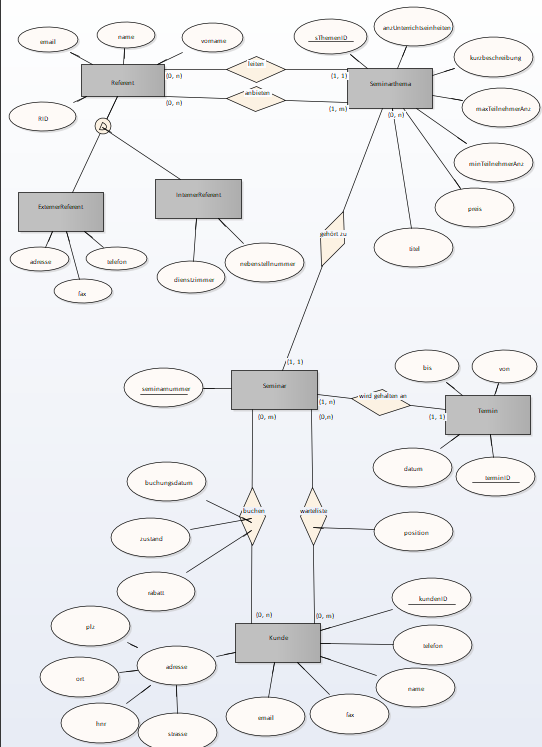
\includegraphics[scale=0.7]{Bilder/ER-Modell.PNG}
	\caption{ER-Modell Seminarverwaltung}
	\label{er:1}
\end{figure}

\subsubsection{Entities}
seminar = (\{\underline{SEMINARNUMMER:INTEGER}\})

termin  = (\{\underline{TERMINID:INTEGER}, DATUM:DATE, VON:DATETIME, BIS:DATETIME\})

kunde   = (\{\underline{KUNDENID:INTEGER}, TELEFON:VARCHAR, NAME:VARCHAR, FAX:VARCHAR, EMAIL:VARCHAR, ADRESSE:(PLZ:VARCHR, ORT:VARCHAR, HNR:VARCHAR, STR:VARCHAR)\})

referent = (\{\underline{RID:INTEGER}, email: VARCHAR, name: VARCHAR, vorname: VARCHAR\})

seminarthema = (\underline{STHEMAID:INTEGER}, ANZUNTERICHTSEINHEITEN:INTEGER, KURZBESCHREIBUNG:VARCHAR, MAXTEILNEHMERANZ:INTEGER, MINTEILNEHMERANZ:INTEGER, PREIS:FLOAT, TITEL:VARCHAR\})

externerReferent = (\{\underline{RID:INTEGER},adresse: (plz: VARCHAR, ort: VARCHAR, strasse: VARCHAR, hnr: VARCHAR)\} is\_a referent)

internerReferent = (\{\underline{RID:INTEGER},dienstzimmer: VARCHAR, nebenstellnummer: Integer\} is\_a referent)

\subsubsection{Relations}

leiten = (referent X seminarthema)

anbieten = (referent X seminarthema)

gehört\_zu = (seminarthema X seminar)

buchen = (seminar x kunke, BUCHUNGSDATUM:DATE, ZUSTAND:VARCHAR, RABATT:FLOAT)

warteliste = (kunde x seminar, POSITION:INTEGER)

wird\_gehalten\_an = (seminar x termin)


\subsection{b)}
\subsubsection{Relationen}
referent = (\underline{RID:INTEGER}, email: VARCHAR, name: VARCHAR, vorname: VARCHAR)

ExternerReferent(\underline{RID:INTEGER}, plz: VARCHAR, ort: VARCHAR, strasse: VARCHAR, hnr: VARCHAR)

IntererReferent (\underline{RID:INTEGER}, dienstzimmer: VARCHAR, nebenstellnummer: Integer) 

seminarthema = (\underline{STHEMAID:INTEGER}, ANZUNTERICHTSEINHEITEN:INTEGER, KURZBESCHREIBUNG:VARCHAR, MAXTEILNEHMERANZ:INTEGER, MINTEILNEHMERANZ:INTEGER, PREIS:FLOAT, TITEL:VARCHAR, LEITER:INTEGER)

anbieten = (\underline{REFERENTID:INTEGER, SEMINARTHEMAID:INTEGER})

seminar = (\underline{SEMINARNUMMER:INTEGER}, SEMINARTHEMAID:INTEGER)

termin = (\underline{TERMINID:INTEGER}, VON:DATETIME, BIS:DATETIME, DATUM:DATE, SEMINARID:INTEGER)

kunde   = (\underline{KUNDENID:INTEGER}, TELEFON:VARCHAR, NAME:VARCHAR, FAX:VARCHAR, EMAIL:VARCHAR, PLZ:VARCHR, ORT:VARCHAR, HNR:VARCHAR, STR:VARCHAR)

buchen = (\underline{KUNDENID:INTEGER, SEMINARNR:INTEGER}, BUCHUNGSDATUM:DATE, ZUSTAND:VARCHAR, RABATT:FLOAT)

warteliste = (\underline{KUNDENID:INTEGER, SEMINARNR:INTEGER}, POSTION:INTEGER)

\subsubsection{Referenzen}
$seminarthema\vert_{LEITER} \subseteq refernet\vert_{RID}$

$anbieten\vert_{REFERENTID} \subseteq refernet\vert_{RID}$

$anbieten\vert_{SEMINARTHEMAID} \subseteq seminarthema\vert_{STHEMAID}$

$seminar\vert_{SEMINARTHEMAID} \subseteq seminarthema\vert_{STHEMAID}$

$termin\vert_{SEMINARID} \subseteq seminar\vert_{SEMINARNUMMER}$

$buchen\vert_{KUNDENID} \subseteq kunde\vert_{KUNDENID}$

$buchen\vert_{SEMINARNR} \subseteq seminar\vert_{SEMINARNR}$

$warteliste\vert_{KUNDENID} \subseteq kunde\vert_{KUNDENID}$

$warteliste\vert_{SEMINARNR} \subseteq seminar\vert_{SEMINARNR}$

\subsection{c)}

\lstinputlisting{../create_table_statements.sql}

\section{2}
\lstinputlisting{../insert_table_statements.sql}

\end{document}



